\section{Results}\label{sec:results}

\subsection{The size of the gap}\label{sec:gap}
Table~\ref{tab:headline} and Figure~\ref{fig:heatmap} summarise the seven-corpus veracity matrix. With \textsc{tfidf-lr}, mean in-domain ROC-AUC is \InAUC{}, mean off-diagonal AUC is \OffAUC{}, and on the eight same-task cells it is \PairAUC{}. The sanity controls behave as they should. With permuted labels, transfer AUC is \PermAUC{} ($\pm$\PermAUCsd{} across cells and seeds) and in-domain AUC \PermInAUC{}. With every source cut to 250 training items the gap remains (in-domain \MatchedInAUC{}, off-diagonal \MatchedOffAUC{}), so it does not come from the very different corpus sizes.

The gap is real, but it is not a collapse to chance. On the cleanest pair, ISOT$\to$WELFake, AUC is \pairISOTWELFakeAUC{} \pairISOTWELFakeCI{}, and in the reverse direction \pairWELFakeISOTAUC{} \pairWELFakeISOTCI{} (Table~\ref{tab:pairs}). Two pairs carry almost no transferable ranking: PolitiFact$\to$LIAR (\pairPFLIARAUC{} \pairPFLIARCI{}) and LIAR$\to$PolitiFact (\pairLIARPFAUC{} \pairLIARPFCI{}). Both are labelled by the same fact-checker, but one rates claims and the other news stories. In \NcellsBelowHalf{} of the 42 off-diagonal cells (\CellsBelowHalf) the mean AUC is below 0.5, meaning that the cue a source teaches points the wrong way on that target.

\begin{table}[t]
\centering
\caption{In-domain versus transfer performance on the seven veracity corpora (mean $\pm$ s.d.\ over seeds of the per-seed mean over cells). ``Pairs'' averages the eight directed same-task cells. Off-diagonal macro-F1 is given at the default threshold and at the oracle threshold. \textsc{roberta-lr} is evaluated on the 1{,}500-item subsets and \textsc{roberta-ft} on 800 training and 300 test items per corpus with three seeds (Section~\ref{sec:models}); compare each with its paired \textsc{tfidf-lr} in Section~\ref{sec:models-res}, not with the rows above.}\label{tab:headline}
\small
\setlength{\tabcolsep}{4pt}
\begin{tabular}{@{}llcccccc@{}}
\toprule
 & & \multicolumn{3}{c}{ROC-AUC} & \multicolumn{3}{c}{macro-F1} \\
\cmidrule(lr){3-5}\cmidrule(lr){6-8}
Model & Regime & In-domain & Off-diag. & Pairs & In-domain & Off-diag. & Off-diag.\ oracle \\
\midrule
\textsc{tfidf-lr} & full & 0.914\,{\scriptsize$\pm$0.006} & 0.567\,{\scriptsize$\pm$0.006} & 0.624\,{\scriptsize$\pm$0.004} & 0.854\,{\scriptsize$\pm$0.005} & 0.439\,{\scriptsize$\pm$0.011} & 0.565\,{\scriptsize$\pm$0.004} \\
\textsc{tfidf-lr} & matched & 0.861\,{\scriptsize$\pm$0.010} & 0.556\,{\scriptsize$\pm$0.004} & 0.590\,{\scriptsize$\pm$0.009} & 0.786\,{\scriptsize$\pm$0.012} & 0.446\,{\scriptsize$\pm$0.014} & 0.558\,{\scriptsize$\pm$0.002} \\
\textsc{tfidf-lr} & permuted & 0.519\,{\scriptsize$\pm$0.026} & 0.499\,{\scriptsize$\pm$0.012} & 0.514\,{\scriptsize$\pm$0.019} & 0.397\,{\scriptsize$\pm$0.014} & 0.377\,{\scriptsize$\pm$0.015} & 0.518\,{\scriptsize$\pm$0.007} \\
\addlinespace
\textsc{tfidf-svm} & full & 0.914\,{\scriptsize$\pm$0.005} & 0.564\,{\scriptsize$\pm$0.005} & 0.625\,{\scriptsize$\pm$0.005} & 0.855\,{\scriptsize$\pm$0.005} & 0.437\,{\scriptsize$\pm$0.009} & 0.564\,{\scriptsize$\pm$0.004} \\
\textsc{tfidf-svm} & matched & 0.862\,{\scriptsize$\pm$0.010} & 0.554\,{\scriptsize$\pm$0.005} & 0.592\,{\scriptsize$\pm$0.010} & 0.787\,{\scriptsize$\pm$0.011} & 0.447\,{\scriptsize$\pm$0.017} & 0.556\,{\scriptsize$\pm$0.003} \\
\textsc{tfidf-svm} & permuted & 0.519\,{\scriptsize$\pm$0.024} & 0.498\,{\scriptsize$\pm$0.015} & 0.511\,{\scriptsize$\pm$0.020} & 0.398\,{\scriptsize$\pm$0.009} & 0.377\,{\scriptsize$\pm$0.012} & 0.516\,{\scriptsize$\pm$0.008} \\
\addlinespace
\textsc{nb-svm} & full & 0.912\,{\scriptsize$\pm$0.004} & 0.547\,{\scriptsize$\pm$0.006} & 0.590\,{\scriptsize$\pm$0.011} & 0.853\,{\scriptsize$\pm$0.008} & 0.410\,{\scriptsize$\pm$0.008} & 0.555\,{\scriptsize$\pm$0.003} \\
\textsc{nb-svm} & matched & 0.862\,{\scriptsize$\pm$0.011} & 0.540\,{\scriptsize$\pm$0.006} & 0.559\,{\scriptsize$\pm$0.004} & 0.786\,{\scriptsize$\pm$0.012} & 0.398\,{\scriptsize$\pm$0.013} & 0.549\,{\scriptsize$\pm$0.004} \\
\textsc{nb-svm} & permuted & 0.510\,{\scriptsize$\pm$0.023} & 0.494\,{\scriptsize$\pm$0.009} & 0.502\,{\scriptsize$\pm$0.009} & 0.400\,{\scriptsize$\pm$0.003} & 0.383\,{\scriptsize$\pm$0.012} & 0.520\,{\scriptsize$\pm$0.006} \\
\addlinespace
\textsc{glove-lr} & full & 0.864\,{\scriptsize$\pm$0.005} & 0.564\,{\scriptsize$\pm$0.005} & 0.610\,{\scriptsize$\pm$0.005} & 0.782\,{\scriptsize$\pm$0.007} & 0.465\,{\scriptsize$\pm$0.004} & 0.564\,{\scriptsize$\pm$0.004} \\
\textsc{glove-lr} & matched & 0.830\,{\scriptsize$\pm$0.006} & 0.563\,{\scriptsize$\pm$0.010} & 0.592\,{\scriptsize$\pm$0.017} & 0.740\,{\scriptsize$\pm$0.011} & 0.466\,{\scriptsize$\pm$0.010} & 0.564\,{\scriptsize$\pm$0.007} \\
\textsc{glove-lr} & permuted & 0.520\,{\scriptsize$\pm$0.022} & 0.504\,{\scriptsize$\pm$0.026} & 0.494\,{\scriptsize$\pm$0.021} & 0.404\,{\scriptsize$\pm$0.020} & 0.391\,{\scriptsize$\pm$0.012} & 0.525\,{\scriptsize$\pm$0.019} \\
\addlinespace
\textsc{style-gb} & full & 0.745\,{\scriptsize$\pm$0.009} & 0.535\,{\scriptsize$\pm$0.004} & 0.595\,{\scriptsize$\pm$0.008} & 0.679\,{\scriptsize$\pm$0.005} & 0.427\,{\scriptsize$\pm$0.007} & 0.548\,{\scriptsize$\pm$0.003} \\
\textsc{style-gb} & matched & 0.702\,{\scriptsize$\pm$0.008} & 0.526\,{\scriptsize$\pm$0.009} & 0.561\,{\scriptsize$\pm$0.032} & 0.632\,{\scriptsize$\pm$0.008} & 0.413\,{\scriptsize$\pm$0.017} & 0.542\,{\scriptsize$\pm$0.007} \\
\textsc{style-gb} & permuted & 0.503\,{\scriptsize$\pm$0.018} & 0.502\,{\scriptsize$\pm$0.016} & 0.493\,{\scriptsize$\pm$0.028} & 0.410\,{\scriptsize$\pm$0.008} & 0.390\,{\scriptsize$\pm$0.007} & 0.523\,{\scriptsize$\pm$0.011} \\
\addlinespace
\textsc{roberta-lr} & full & 0.861\,{\scriptsize$\pm$0.012} & 0.544\,{\scriptsize$\pm$0.008} & 0.630\,{\scriptsize$\pm$0.011} & 0.777\,{\scriptsize$\pm$0.013} & 0.452\,{\scriptsize$\pm$0.013} & 0.549\,{\scriptsize$\pm$0.010} \\
\addlinespace
\textsc{roberta-ft} & full & 0.867\,{\scriptsize$\pm$0.010} & 0.559\,{\scriptsize$\pm$0.013} & 0.614\,{\scriptsize$\pm$0.020} & 0.795\,{\scriptsize$\pm$0.005} & 0.418\,{\scriptsize$\pm$0.009} & 0.571\,{\scriptsize$\pm$0.008} \\
\bottomrule
\end{tabular}
\end{table}


\begin{figure}[t]
\centering
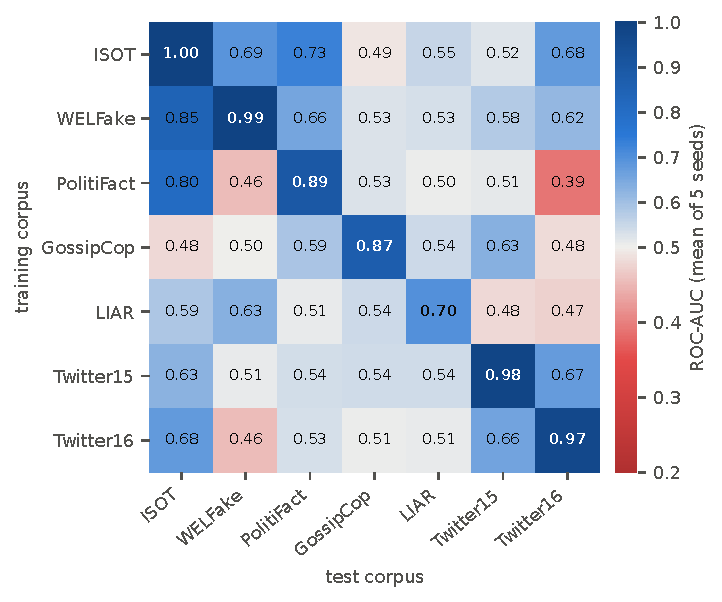
\includegraphics[width=0.62\linewidth]{fig_heatmap_auc}
\caption{Transfer ROC-AUC of \textsc{tfidf-lr} (mean of five seeds). Rows are training corpora, columns test corpora; the diagonal is in-domain. Blue is above chance, red below; the midpoint is 0.5.}\label{fig:heatmap}
\end{figure}

\begin{table}[t]
\centering
\caption{Same-task pairs (\textsc{tfidf-lr}, five seeds). AUC with pooled seed-bootstrap 95\% CI; ``In'' is the source's in-domain AUC; prior is the target fake rate and PPR the predicted-positive rate at $t=0.5$; macro-F1 at the default, prior-matched and oracle thresholds; ECE of the source-calibrated scores on the target.}\label{tab:pairs}
\small
\begin{tabular}{@{}lcccccccc@{}}
\toprule
Pair & In & AUC [95\% CI] & Prior & PPR & F1$_{0.5}$ & F1$_{\pi}$ & F1$^\star$ & ECE \\
\midrule
ISOT$\to$WELFake & 0.999 & 0.690 [0.66, 0.71] & 0.43 & 0.78 & 0.539 & 0.635 & 0.638 & 0.38 \\
WELFake$\to$ISOT & 0.989 & 0.847 [0.82, 0.87] & 0.46 & 0.36 & 0.753 & 0.763 & 0.765 & 0.11 \\
PolitiFact$\to$GossipCop & 0.893 & 0.526 [0.48, 0.56] & 0.23 & 0.54 & 0.464 & 0.514 & 0.517 & 0.32 \\
GossipCop$\to$PolitiFact & 0.869 & 0.589 [0.50, 0.68] & 0.43 & 0.07 & 0.425 & 0.576 & 0.595 & 0.28 \\
Twitter15$\to$Twitter16 & 0.981 & 0.672 [0.52, 0.82] & 0.46 & 0.62 & 0.572 & 0.597 & 0.646 & 0.25 \\
Twitter16$\to$Twitter15 & 0.967 & 0.657 [0.55, 0.75] & 0.51 & 0.63 & 0.580 & 0.591 & 0.631 & 0.28 \\
LIAR$\to$PolitiFact & 0.698 & 0.508 [0.42, 0.60] & 0.44 & 0.54 & 0.495 & 0.517 & 0.536 & 0.12 \\
PolitiFact$\to$LIAR & 0.893 & 0.505 [0.47, 0.54] & 0.44 & 0.40 & 0.497 & 0.502 & 0.509 & 0.22 \\
\bottomrule
\end{tabular}
\end{table}


Threshold-dependent metrics look much worse than AUC. Off-diagonal macro-F1 at the default threshold averages \OffFone{}, not far above the one-class level of 0.33, against \InFone{} in-domain. The predicted-positive rates in Table~\ref{tab:pairs} show why. An ISOT model flags \pairISOTWELFakePPR{} of WELFake as fake although the fake rate is \pairISOTWELFakePrior{}, and a GossipCop model flags only \pairGCPFPPR{} of PolitiFact although its fake rate is \pairGCPFPrior{}. Scores that were well calibrated in-domain are badly calibrated on the target.

\subsection{Where the gap goes}\label{sec:where}
Applying Eq.~\eqref{eq:decomp} cell by cell (Table~\ref{tab:decomp}, Figure~\ref{fig:decomp}) splits the loss into a part that no threshold can recover and a part that the right threshold would. For \textsc{tfidf-lr} on the same-task pairs, the mean transfer gap is \GapPair{} macro-F1 points, of which \RankPair{} (\RankSharePair) is a ranking deficit and the rest an operating-point loss. On the other cells the gap is \GapOther{}, and \RankShareOther{} of it is ranking. Over all cells, \RankShareAll{} of the loss is ranking (corpus-bootstrap 95\% interval \RankShareCI) and \OpShareAll{} is operating point. Most of the gap is ranking, then, and part of it is threshold. Both parts matter. The operating-point share is large enough to change which of two detectors looks better, and it is the cheaper one to fix.

\begin{table}[t]
\centering
\caption{Transfer gap decomposition (Eq.~\ref{eq:decomp}), macro-F1 points, mean over cells and seeds. The gap is relative to the target's own in-domain score.}\label{tab:decomp}
\small
\begin{tabular}{@{}llrrrrr@{}}
\toprule
Model & Cells & Gap & Ranking & Threshold & Prior/cal. & Ranking share \\
\midrule
\textsc{tfidf-lr} & pairs & 0.308 & 0.244 & 0.018 & 0.046 & 79\% \\
\textsc{tfidf-lr} & other cells & 0.441 & 0.300 & 0.018 & 0.122 & 68\% \\
\textsc{tfidf-svm} & pairs & 0.308 & 0.243 & 0.016 & 0.049 & 79\% \\
\textsc{tfidf-svm} & other cells & 0.444 & 0.303 & 0.018 & 0.123 & 68\% \\
\textsc{nb-svm} & pairs & 0.319 & 0.261 & 0.023 & 0.036 & 82\% \\
\textsc{nb-svm} & other cells & 0.472 & 0.306 & 0.021 & 0.145 & 65\% \\
\textsc{glove-lr} & pairs & 0.281 & 0.193 & 0.016 & 0.071 & 69\% \\
\textsc{glove-lr} & other cells & 0.327 & 0.224 & 0.017 & 0.085 & 69\% \\
\textsc{style-gb} & pairs & 0.141 & 0.091 & 0.013 & 0.036 & 65\% \\
\textsc{style-gb} & other cells & 0.278 & 0.141 & 0.020 & 0.117 & 51\% \\
\textsc{roberta-lr} & pairs & 0.243 & 0.162 & 0.022 & 0.059 & 66\% \\
\textsc{roberta-lr} & other cells & 0.344 & 0.244 & 0.024 & 0.076 & 71\% \\
\textsc{roberta-ft} & pairs & 0.340 & 0.186 & 0.031 & 0.123 & 55\% \\
\textsc{roberta-ft} & other cells & 0.387 & 0.233 & 0.027 & 0.127 & 60\% \\
\bottomrule
\end{tabular}
\end{table}


\begin{figure}[t]
\centering
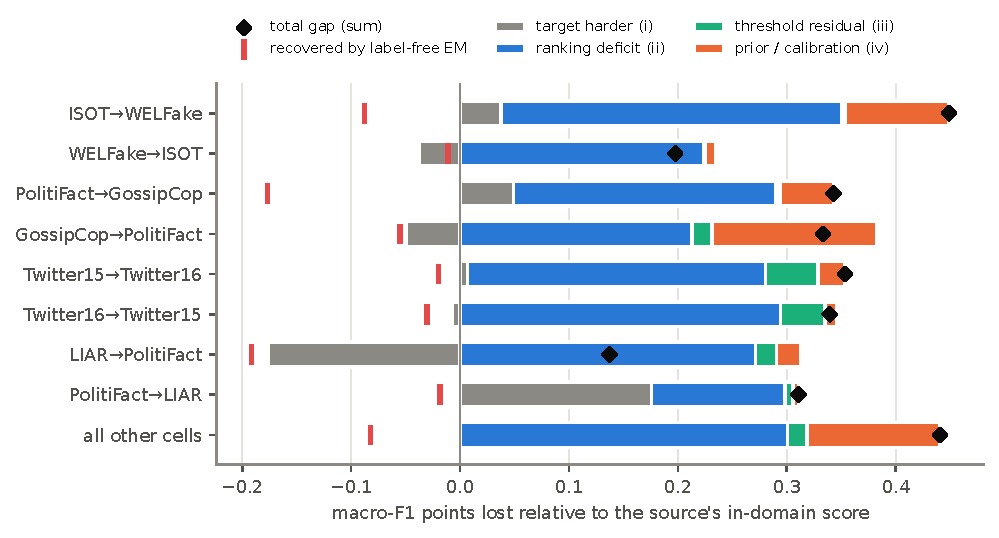
\includegraphics[width=\linewidth]{fig_gap_decomposition}
\caption{Transfer gap decomposition for \textsc{tfidf-lr} (macro-F1 points relative to the source's in-domain score, mean of five seeds). Grey: target harder or easier than source; blue: ranking deficit; green and orange: operating-point losses. Diamonds mark the total; red ticks show what EM prior adaptation recovers (negative values make things worse).}\label{fig:decomp}
\end{figure}

\subsection{How robust is the split?}\label{sec:robust}
The split survives every check we ran. Dropping any one corpus from the matrix leaves the ranking share between \RankShareDropMin{} and \RankShareDropMax. The in-domain threshold slack that the ranking term absorbs is small, \SlackFone{} macro-F1 on average (at most \SlackFoneMax). The in-sample oracle is optimistic, as expected: a threshold tuned on one half of the target and scored on the other reaches \OracleCF{}, which is \OracleCFbias{} below the in-sample oracle on average and \OracleCFbiasSmall{} below it on the targets with fewer than 250 test items. With the cross-fitted oracle the ranking share rises to \RankShareCF{}, so if anything Eq.~\eqref{eq:decomp} overstates the operating-point part. With balanced accuracy in place of macro-F1, the ranking share is \BARankShare{}. Across detectors the ranking share varies more (Table~\ref{tab:decomp}): it is lowest for the style model on the non-paired cells and for the fine-tuned transformer (\FTRankShare{} overall; Section~\ref{sec:models-res}), but ranking is the larger part for every detector.

\subsection{Repairing the operating point without labels}\label{sec:op}
Table~\ref{tab:oppoints} and Figure~\ref{fig:op} compare operating points. EM prior adaptation, the textbook remedy, \emph{lowers} off-diagonal macro-F1 from \OPDef{} to \OPEM{}. It recovers \RecEM{} of the operating-point loss (interval \RecEMCI), and it does so for every detector (\RecEMMin{} to \RecEMMax). Rate transfer, which flags the same share of target items as the source base rate, raises macro-F1 to \OPRank{} and recovers \RecRank{} (\RecRankCI), close to the \RecPrior{} reached when the true target base rate is known (\OPPrior{}). It recovers between \RecRankMin{} and \RecRankMax{} across the seven detectors, and it is at least as good as the cross-fitted oracle, that is, as a threshold tuned on half of the labelled target set (recovery \RecRankCF{} against that oracle). Flagging the share $q_A$ that the source model flags in-domain recovers \RecSrcPPR, and the mixture model \RecGMM. Rate transfer is worse than the default threshold in \RankWorseShare{} of the cell-seed combinations.

Two observations keep these numbers in proportion. First, flagging exactly half of the items recovers \RecHalf{}, almost as much as rate transfer. The source base rates of our corpora lie between 0.23 and 0.51, so in this benchmark most of the gain comes from switching from a score threshold to \emph{any} sensible rate threshold, and only a small part from knowing the source rate. Second, the source base rate is a good guess of the target base rate here (mean absolute error \SrcPriorErr), which is condition (ii) of Proposition~\ref{prop:rate}.

Why does EM fail? The answer is in the calibration. EM is optimal when only $p(y)$ changes and calibrated posteriors stay meaningful. Here calibration does not survive the move: expected calibration error is \ECEin{} in-domain but \ECEout{} on the target. EM's prior estimates therefore drift towards 0 or 1 (mean absolute error \EMpriorErr), far worse than simply assuming the source prior (\SrcPriorErr). Adjusted classify-and-count fails for the same reason, because the source error rates it inverts do not hold on the target either (prior error \ErrACC, recovery \RecACC). The shift is in $p(x\mid y)$, that is, in style, topic and source, much more than in $p(y)$. That is the regime in which Proposition~\ref{prop:rate} favours transferring the rate over transferring the scores.

\begin{table}[t]
\centering
\caption{Off-diagonal macro-F1 under different operating points (mean over the 42 cells and five seeds). Label-free: default $t=0.5$, EM prior adaptation, rate transfer (predicted-positive rate set to the source base rate), predicted-positive rate 0.5, and a 2-component GMM on target logits. With one number known: rate set to the true target prior. Upper bound: oracle threshold. For \textsc{tfidf-lr}, Holm-corrected Wilcoxon $p$ versus default: EM 1.6e-32, rate transfer 6.6e-31, rate 0.5 1.4e-29, GMM 1.7e-18.}\label{tab:oppoints}
\small
\begin{tabular}{@{}lccccccc@{}}
\toprule
 & \multicolumn{5}{c}{label-free} & prior known & bound \\
\cmidrule(lr){2-6}\cmidrule(lr){7-7}\cmidrule(lr){8-8}
Model & $t=0.5$ & EM & rate transfer & rate 0.5 & GMM & rate $=\pi_B$ & oracle \\
\midrule
\textsc{tfidf-lr} & 0.439 & 0.358 & 0.541 & 0.539 & 0.510 & 0.547 & 0.565 \\
\textsc{tfidf-svm} & 0.437 & 0.363 & 0.539 & 0.537 & 0.503 & 0.546 & 0.564 \\
\textsc{nb-svm} & 0.410 & 0.349 & 0.525 & 0.526 & 0.444 & 0.534 & 0.555 \\
\textsc{glove-lr} & 0.465 & 0.381 & 0.540 & 0.542 & 0.494 & 0.547 & 0.564 \\
\textsc{style-gb} & 0.427 & 0.347 & 0.521 & 0.521 & 0.477 & 0.529 & 0.548 \\
\textsc{roberta-lr} & 0.452 & 0.368 & 0.516 & 0.516 & 0.477 & 0.525 & 0.549 \\
\textsc{roberta-ft} & 0.418 & 0.340 & 0.535 & 0.534 & 0.479 & 0.544 & 0.571 \\
\bottomrule
\end{tabular}
\end{table}


\begin{figure}[t]
\centering
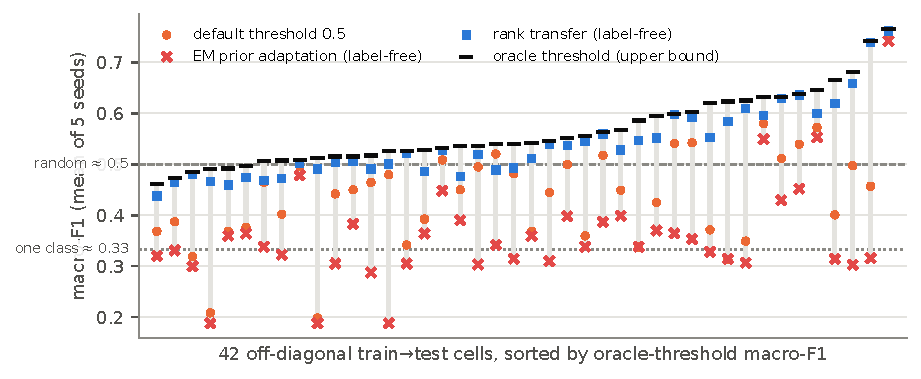
\includegraphics[width=\linewidth]{fig_operating_points}
\caption{Off-diagonal macro-F1 of \textsc{tfidf-lr} for each of the 42 cells (mean of five seeds), sorted by the oracle bound. Rate transfer closes most of the distance from the default threshold to the oracle without any target label; EM prior adaptation often falls below the default.}\label{fig:op}
\end{figure}

\paragraph{When the base rate moves}
Condition (ii) will not always hold, so we resampled every target to base rates between 0.3 below and 0.3 above the source rate (Figure~\ref{fig:priorshift}). Rate transfer degrades as the shift grows: it recovers \PSrecZero{} of the operating-point loss with no shift, \PSrecMinus{} at $-0.3$ and \PSrecPlus{} at $+0.3$, where its macro-F1 (\PSrankPlus) falls well below that of a threshold set at the true rate (\PStruePlus). It still beats the default threshold at every shift we tried, by \PSgainMin{} to \PSgainMax{} macro-F1. The two label-free prior estimators do not help: EM and adjusted classify-and-count stay below the default threshold at every shift, because both rely on score distributions that do not transfer. In practice, then, rate transfer is a safe default, but when the base rate of the new feed is expected to differ from the training data, an estimate of that rate from a small labelled sample is worth more than any label-free correction we tested.

\begin{figure}[t]
\centering
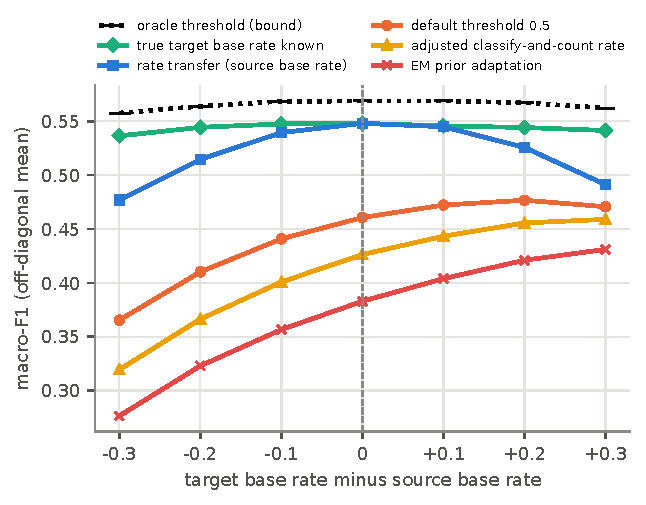
\includegraphics[width=0.66\linewidth]{fig_prior_shift}
\caption{Off-diagonal macro-F1 of \textsc{tfidf-lr} when every target test set is resampled to the source base rate plus a shift (42 cells, five seeds, three draws of 1{,}000 items). Rate transfer is best when the base rate is unchanged and degrades as it moves; the label-free prior estimators (EM, adjusted classify-and-count) stay below the default threshold throughout.}\label{fig:priorshift}
\end{figure}

\subsection{The gap across models}\label{sec:models-res}
The picture does not depend on the detector (Table~\ref{tab:headline}; full matrices for every model are in the Supplementary Material). The four content models reach in-domain AUC between \InAUCmin{} and \InAUCmax{} and off-diagonal AUC between \OffAUCmin{} and \OffAUCmax{}, and all of them show the same split between ranking and operating-point loss (Table~\ref{tab:decomp}). Averaged word embeddings (\textsc{glove-lr}) are weaker in-domain (\GloveInAUC) and transfer no better (\GloveOffAUC).

The style model is the most revealing. With only 22 surface statistics it reaches an average in-domain AUC of \StyleInAUC{} (\StyleISOT{} on ISOT, \StyleWEL{} on WELFake), and its transfer AUC (\StyleOffAUC) is only a few points below that of the lexical models. A large part of what these benchmarks reward is form: length, casing, punctuation and attribution habits (Section~\ref{sec:shortcuts}).

Pretrained encoders do not change the conclusion. On identical 1{,}500-item subsets, frozen RoBERTa features give in-domain AUC \RobInAUC{} and off-diagonal AUC \RobOffAUC{}, against \SubLRInAUC{} and \SubLROffAUC{} for \textsc{tfidf-lr} refitted on the same splits. The paired off-diagonal difference is \RobMinusLRoff{} AUC (Wilcoxon $p=\RobMinusLRp$), and RoBERTa is better in \RobBetterCells{} of the 42 cells. Fine-tuning the upper four layers does not change this either. On the same 800 training and 300 test items per corpus (\FTseeds{} seeds), \textsc{roberta-ft} reaches in-domain AUC \FTInAUC{} and off-diagonal AUC \FTOffAUC{}, against \FTsubInAUC{} and \FTsubOffAUC{} for the paired \textsc{tfidf-lr}; the off-diagonal difference is \FTminusLRoff{} (Wilcoxon $p=\FTminusLRp$, better in \FTbetterCells{} of 42 cells). Its gap is again mostly ranking (\FTRankShare), EM again makes the operating point worse (\FTRecEM{} recovered), and rate transfer again recovers most of it (\FTRecRank). With only four layers trained on 800 items, the fine-tuned model is slightly weaker than \textsc{tfidf-lr} in-domain (\FTminusLRin{} AUC), so this is not the strongest transformer one could build; but its transfer matches that of the lexical model, and the shape of its gap is the same. This agrees with \citet{verma2026audit} and \citet{delloglio2026comparison}, who found that fully fine-tuned transformers gain in-domain but not, or not reliably, across corpora. Pairwise McNemar tests on the same target items (Holm-corrected over all comparisons) find significant differences from \textsc{tfidf-lr} in the following share of (cell, seed) comparisons: \McFracSig.

\subsection{What the detectors learn}\label{sec:shortcuts}
\paragraph{Cheap signals go a long way}
Table~\ref{tab:shortcuts} lists four shortcut indicators per corpus. The surface-statistics model recovers on average \StyleShare{} of the above-chance in-domain AUC of the full lexical model, and on the article corpora almost all of it (ISOT \StyleISOT, WELFake \StyleWEL). Sixty-four training examples are enough for an in-domain AUC of \LCsixfourISOT{} on ISOT and \LCsixfourWEL{} on WELFake; the claim and celebrity-headline corpora, whose in-domain scores are lower to begin with, learn much more slowly (LIAR \LCsixfourLIAR, GossipCop \LCsixfourGC). On the headline and claim corpora, publisher or speaker identity alone predicts the label with AUC \GroupPF{} (PolitiFact), \GroupGC{} (GossipCop) and \GroupLIAR{} (LIAR). A label that can be predicted from form, from a few dozen examples or from who published an item is a label whose in-domain score says little about veracity.

\begin{table}[t]
\centering
\caption{Shortcut indicators (ROC-AUC, mean of five seeds). In-domain AUC of \textsc{tfidf-lr} with the full training split, of the surface-statistics \textsc{style-gb}, and of \textsc{tfidf-lr} trained on only 64 or 256 items; AUC of a group-identity baseline (publisher domain for PolitiFact and GossipCop, speaker for LIAR); and the mean off-diagonal AUC with the corpus as source and as target.}\label{tab:shortcuts}
\small
\begin{tabular}{@{}lccccccc@{}}
\toprule
 & \multicolumn{5}{c}{in-domain} & \multicolumn{2}{c}{transfer} \\
\cmidrule(lr){2-6}\cmidrule(lr){7-8}
Corpus & full & style only & $n=64$ & $n=256$ & group only & as source & as target \\
\midrule
ISOT & 0.999 & 0.999 & 0.983 & 0.991 & -- & 0.611 & 0.670 \\
WELFake & 0.989 & 0.951 & 0.894 & 0.941 & -- & 0.626 & 0.540 \\
PolitiFact & 0.893 & 0.787 & 0.742 & 0.850 & 0.840 & 0.533 & 0.592 \\
GossipCop & 0.869 & 0.659 & 0.610 & 0.723 & 0.807 & 0.538 & 0.522 \\
LIAR & 0.698 & 0.590 & 0.567 & 0.607 & 0.664 & 0.537 & 0.530 \\
Twitter15 & 0.981 & 0.603 & 0.793 & 0.962 & -- & 0.572 & 0.563 \\
Twitter16 & 0.967 & 0.625 & 0.890 & -- & -- & 0.556 & 0.552 \\
\bottomrule
\end{tabular}
\end{table}


\paragraph{The strongest cues are collection signatures}
Figure~\ref{fig:weights} shows the highest-weight n-grams. In ISOT, the real class is signalled by Reuters wire conventions (``reuters'', ``said'', ``washington reuters'', weekday attributions such as ``on thursday'') and the fake class by the template of the sites it was collected from (``featured image'', ``image via'', ``read more'', ``video''). In WELFake, the real class is signalled by publisher suffixes inherited from one of its source collections (``breitbart'', ``york times'', ``mr'') and the fake class by the window in which fake items were gathered (``2016'', ``october'', ``november'', ``hillary''). Each corpus thus teaches a different, corpus-specific proxy, which explains why the sign of a cue can flip from one corpus to another (Section~\ref{sec:gap}).

\begin{figure}[t]
\centering
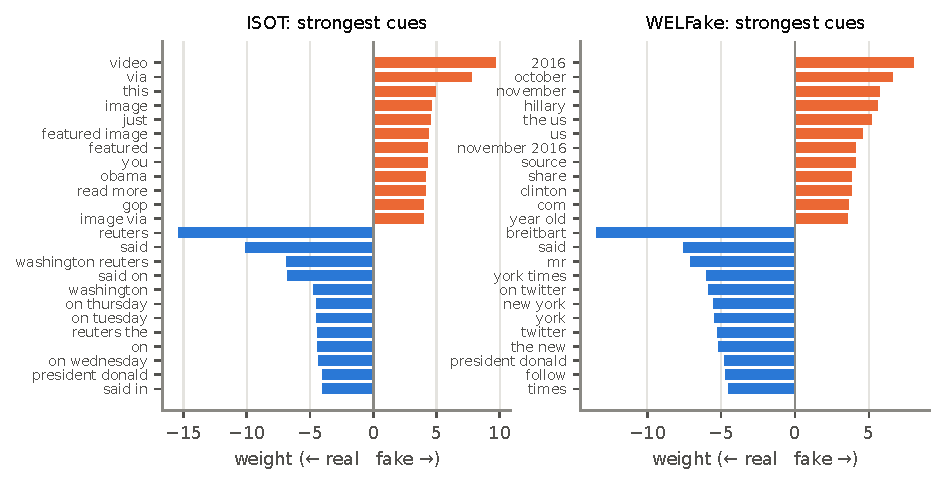
\includegraphics[width=\linewidth]{fig_weights}
\caption{Highest-weight n-grams of \textsc{tfidf-lr} (seed 0) for the real (blue) and fake (orange) classes. Both corpora are separated mainly by outlet conventions and collection-period vocabulary.}\label{fig:weights}
\end{figure}

\paragraph{Removing cues does not remove the signal}
Deleting the top-$K$ features and retraining barely moves in-domain AUC: on ISOT it goes from \TopKISOTIn{} with all features to \TopKISOTInThousand{} after deleting 1{,}000 and \TopKISOTInMax{} after 3{,}000, and on WELFake from \TopKWELIn{} to \TopKWELInThousand{} and \TopKWELInMax{}; transfer to the paired corpus, in contrast, falls from \TopKISOTPair{} to \TopKISOTPairMax{} (ISOT$\to$WELFake) and from \TopKWELPair{} to \TopKWELPairMax{} (WELFake$\to$ISOT). The highest-weight features thus carry most of what transfers, while the signal that keeps in-domain AUC near its ceiling is spread over thousands of corpus-specific features. Masking source tags, datelines, time expressions, numbers and named entities together (Table~\ref{tab:mask}) leaves in-domain AUC at \MaskISOTAllIn{} (ISOT) and \MaskWELAllIn{} (WELFake), and moves ISOT$\to$WELFake from \MaskISOTNonePair{} to \MaskISOTAllPair{} and WELFake$\to$ISOT from \MaskWELNonePair{} to \MaskWELAllPair{}. Balancing classes within each of 50 topic clusters, whose class purity averages \TopicISOTPurity{} in ISOT and \TopicWELPurity{} in WELFake, leaves in-domain AUC unchanged (ISOT \TopicISOTRandIn{}$\to$\TopicISOTBalIn{}, WELFake \TopicWELRandIn{}$\to$\TopicWELBalIn{}) and transfer unchanged (\TopicISOTRandOut{}$\to$\TopicISOTBalOut{}, \TopicWELRandOut{}$\to$\TopicWELBalOut{}); only GossipCop loses in-domain AUC (\TopicGCRandIn{}$\to$\TopicGCBalIn{}). The separating signal is therefore diffuse: it lives in style and register throughout the text, not in a removable list of tokens or topics, as \citet{verma2026audit} also found for ISOT.

\begin{table}[t]
\centering
\caption{Masking ablation (\textsc{tfidf-lr}, ROC-AUC, three seeds, first 3{,}000 characters). Rows: training corpus and what is masked in every corpus; columns: test corpus (the training corpus's own column is in-domain).}\label{tab:mask}
\small
\begin{tabular}{@{}llccccc@{}}
\toprule
Train & Masked & ISOT & WELFake & PolitiFact & GossipCop & LIAR \\
\midrule
ISOT & none & 0.998 & 0.679 & 0.739 & 0.481 & 0.559 \\
ISOT & source tags, datelines, URLs, handles & 0.997 & 0.681 & 0.733 & 0.483 & 0.559 \\
ISOT & dates, weekdays, numbers & 0.998 & 0.692 & 0.723 & 0.479 & 0.563 \\
ISOT & named entities & 0.996 & 0.657 & 0.678 & 0.543 & 0.557 \\
ISOT & all of the above & 0.996 & 0.650 & 0.678 & 0.540 & 0.556 \\
\addlinespace
WELFake & none & 0.808 & 0.980 & 0.636 & 0.529 & 0.532 \\
WELFake & source tags, datelines, URLs, handles & 0.815 & 0.979 & 0.634 & 0.533 & 0.536 \\
WELFake & dates, weekdays, numbers & 0.831 & 0.977 & 0.608 & 0.509 & 0.526 \\
WELFake & named entities & 0.833 & 0.965 & 0.614 & 0.511 & 0.522 \\
WELFake & all of the above & 0.810 & 0.964 & 0.611 & 0.500 & 0.522 \\
\bottomrule
\end{tabular}
\end{table}


\paragraph{Corpus divergence does not predict transfer}
Every pair of corpora can be told apart from text alone (proxy $\mathcal{A}$-distance between \PADmin{} and \PADmax{}, maximum 2; ISOT--WELFake \PADiw), yet across the 42 cells we find no association between source--target divergence and transfer AUC (Spearman $\rho=\PADrho$). With seven corpora the corpus-bootstrap 95\% interval is wide (\PADrhoCI), so a moderate association cannot be excluded, but label-free divergence is clearly not a usable predictor of transfer here. Transfer depends less on how different two corpora look than on whether the cue that separates the classes in one also separates them, with the same sign, in the other.

\subsection{Repairing the ranking}\label{sec:repair-res}
Table~\ref{tab:repair} reports the leave-one-corpus-out repairs (per-target values in Table~\ref{tab:repair-targets}). Training on the six other corpora at once is the one change that helps ranking: held-out AUC rises to \LocoPooled{}, against \LocoMeanSingle{} for the average single source. This is close to the best single source chosen with hindsight (\LocoBestSingle), which cannot be identified without target labels, and far below the targets' own in-domain AUC of \LocoCeiling{}. Nothing we add on top of pooling helps on average. Balancing every (corpus, class) cell (\LocoBal, $\Delta$\LocoBalDelta, $p=\LocoBalP$) and masking collection signatures (\LocoMask, $\Delta$\LocoMaskDelta, $p=\LocoMaskP$) leave AUC unchanged on average; masking helps clearly only on ISOT (Table~\ref{tab:repair-targets}), the corpus whose signatures it was written for.

Methods that make the representation \emph{invariant to corpus identity} make ranking worse: deleting the 2{,}000 most corpus-predictive features gives \LocoDrop{} ($\Delta$\LocoDropDelta, $p=\LocoDropP$), CORAL \LocoCORAL{} ($\Delta$\LocoCORALDelta, $p=\LocoCORALP$) and INLP \LocoINLP{} ($\Delta$\LocoINLPDelta, $p=\LocoINLPP$). INLP does what it is designed to do, reducing linear corpus-identity accuracy from \INLPaccBefore{} to \INLPaccAfter{} (six classes), but it removes veracity information with it. In these benchmarks corpus identity and label are entangled: each corpus collected its fake and real items from different outlets, periods and formats, so the directions that identify a corpus are partly the directions that separate its classes. Invariance to the corpus is therefore not invariance to the shortcut, and the remaining ranking gap is a property of the data rather than of the learner.

\begin{table}[t]
\centering
\caption{Leave-one-corpus-out repairs (\textsc{tfidf-lr} features; mean over the seven held-out veracity corpora and five seeds; s.d.\ across seeds). $\Delta$AUC versus pooled training with Holm-corrected Wilcoxon $p$ over the 35 (target, seed) pairs. For reference, the mean single-source transfer AUC to the same targets is 0.567, the best single source (chosen with target labels) 0.671, and the targets' own in-domain AUC 0.914.}\label{tab:repair}
\small
\begin{tabular}{@{}lccccc@{}}
\toprule
Training & AUC & AP & F1$_{0.5}$ & F1$^\star$ & $\Delta$AUC ($p$) \\
\midrule
pooled (6 corpora) & 0.660\,{\scriptsize$\pm$0.013} & 0.582 & 0.581 & 0.634 & -- \\
+ (corpus, class) balancing & 0.659\,{\scriptsize$\pm$0.013} & 0.583 & 0.582 & 0.632 & -0.001 (1.000) \\
+ balancing + masking & 0.661\,{\scriptsize$\pm$0.012} & 0.584 & 0.576 & 0.633 & +0.001 (1.000) \\
+ balancing + corpus-feature deletion & 0.636\,{\scriptsize$\pm$0.011} & 0.556 & 0.560 & 0.611 & -0.023 (0.006) \\
SVD-300 + balancing & 0.647\,{\scriptsize$\pm$0.009} & 0.566 & 0.583 & 0.624 & -0.013 (0.043) \\
SVD-300 + INLP & 0.605\,{\scriptsize$\pm$0.011} & 0.520 & 0.525 & 0.591 & -0.054 (0.001) \\
SVD-300 + CORAL & 0.621\,{\scriptsize$\pm$0.008} & 0.539 & 0.563 & 0.604 & -0.038 ($<$0.001) \\
\bottomrule
\end{tabular}
\end{table}

\begin{table}[h]
\centering
\caption{Leave-one-corpus-out AUC per held-out corpus (mean of five seeds), against single-source transfer and the in-domain ceiling.}\label{tab:repair-targets}
\small
\begin{tabular}{@{}lccccccc@{}}
\toprule
Held out & mean single & best single & pooled & + masking & INLP & CORAL & in-domain \\
\midrule
ISOT & 0.670 & 0.847 & 0.865 & 0.890 & 0.805 & 0.781 & 0.999 \\
WELFake & 0.540 & 0.690 & 0.648 & 0.657 & 0.643 & 0.643 & 0.989 \\
PolitiFact & 0.592 & 0.730 & 0.677 & 0.655 & 0.600 & 0.650 & 0.893 \\
GossipCop & 0.522 & 0.544 & 0.538 & 0.546 & 0.558 & 0.520 & 0.869 \\
LIAR & 0.530 & 0.552 & 0.528 & 0.528 & 0.502 & 0.514 & 0.698 \\
Twitter15 & 0.563 & 0.657 & 0.647 & 0.645 & 0.592 & 0.626 & 0.981 \\
Twitter16 & 0.552 & 0.678 & 0.715 & 0.703 & 0.536 & 0.616 & 0.967 \\
\bottomrule
\end{tabular}
\end{table}


\subsection{A low-resource language: Bengali clickbait}\label{sec:bangla}
\paragraph{Replication and duplicates}
On the official BanglaBait split, character 3--5-gram logistic regression reaches a clickbait-class F1 of \BBrelFone{} (Figure~\ref{fig:bengali}a), within two points of the 66.28 reported for the same model by \citet{mahtab2023banglabait}, and a linear SVM reaches \BBrelSVMFone{}. Removing the near-duplicates found by MinHash from the official splits lowers the same model to \BBdedFone{} (AUC \BBrelAUC{}$\to$\BBdedAUC{}): even after the original authors' Levenshtein filter, duplicated titles inflate the benchmark. Over five random re-splits of the deduplicated corpus the model reaches AUC \BBseedAUC{} $\pm$ \BBseedAUCsd{}.

\paragraph{Publisher identity}
The \BBnPub{} publishers with at least 100 articles have clickbait rates from \BBrateMin{} to \BBrateMax{}, so publisher identity alone predicts the label with AUC \BBgroupAUC{} (Section~\ref{sec:shortcuts}). Leave-one-publisher-out evaluation nevertheless costs little: across \BBlosoN{} held-out publishers (the smallest ones pooled), mean AUC is \BBlosoAUC{} (range \BBlosoMin--\BBlosoMax), close to the random-split value. Bengali clickbait detection survives a change of source that English veracity detection does not. One reading is that this is a construct effect rather than a language effect. Clickbait \emph{is} a property of a headline's style, so a style-sensitive detector can learn the construct itself, whereas for veracity, style is only a correlate of the label that changes from corpus to corpus. The comparison is not fully controlled, though: BanglaBait was labelled by annotators reading each headline, while the English veracity labels come from fact-checks or from the outlet an article was taken from, so how the labels were made differs as well as what they mean.

\paragraph{Across languages}
A translate-test probe uses BanglaBait's machine-translated English titles. A detector trained on English clickbait headlines \citep{chakraborty2016clickbait} ranks translated Bengali titles with AUC \XlENtoBB{}, against \XlBBEN{} for a detector trained on the translated titles themselves and \XlBN{} for one trained on the original Bengali; translation costs about \XlTransCost{} AUC and most of the in-language ranking ability carries over. In the other direction, the translated-Bengali detector reaches \XlBBtoEN{} on English headlines (in-domain \XlEN). Clickbait carries over across languages much better than veracity carries over across English corpora, although translation and the change of collection still cost about 0.1 AUC (\XlENtoBB{} against \XlBN{} in-language).

\begin{figure}[t]
\centering
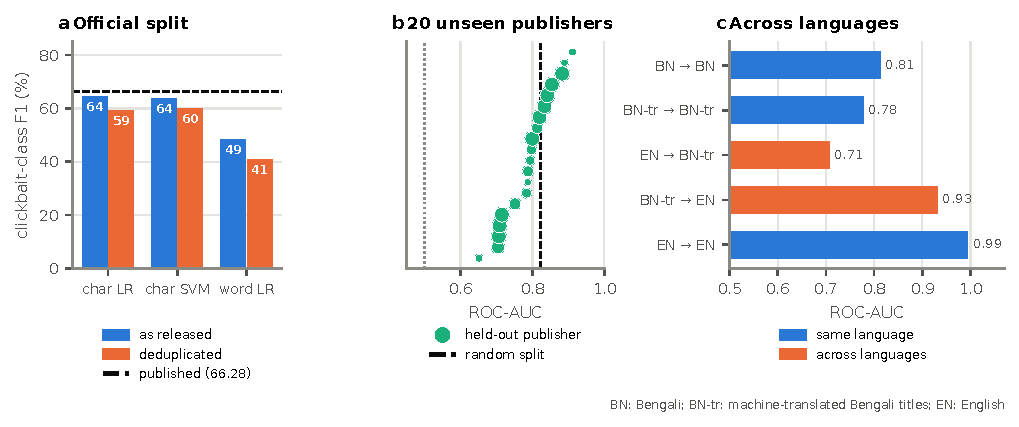
\includegraphics[width=\linewidth]{fig_bengali}
\caption{Bengali clickbait. (a)~Clickbait-class F1 on the official BanglaBait split, as released and after removing near-duplicates, against the published value for character LR \citep{mahtab2023banglabait}. (b)~ROC-AUC on each held-out publisher (dot size: number of articles) against the random-split value. (c)~Translate-test: training and test corpora in Bengali (BN), machine-translated Bengali titles (BN-tr) or English clickbait headlines (EN).}\label{fig:bengali}
\end{figure}

